\documentclass{standalone}
\usepackage[T1]{fontenc}
\usepackage[utf8]{inputenc}
\usepackage{pgf,tikz}
\usetikzlibrary{calc}

\usepackage{setspace}

\begin{document}
\footnotesize
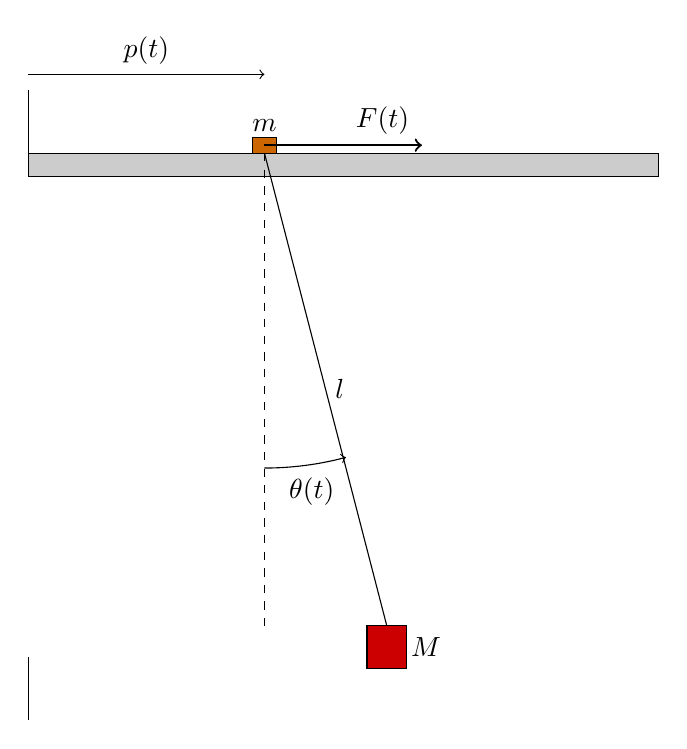
\begin{tikzpicture}[scale=1.0,]
  \def\beamh{0.3}
  \def\beaml{8}
  \def\carth{0.2}
  \def\cartw{0.3}
  \def\cartpos{3}
  \def\thta{15}
  \def\cablel{6}
  \def\contw{0.5}
  \def\conth{0.55}
  \pgfmathsetmacro{\contpos}{\cartpos + \cablel * sin(\thta)}
  \pgfmathsetmacro{\cartleft}{\cartpos -0.5*\cartw}
  \pgfmathsetmacro{\contleft}{\contpos -0.5*\contw}
  \pgfmathsetmacro{\contlower}{-\cablel -\conth}
  
  \draw[fill=black!20] (0, -\beamh) rectangle (\beaml, 0);
  \draw[fill=orange!80!black] (\cartleft, 0) rectangle ++(\cartw, \carth);
  \node at (\cartpos, 0.35) {$m$};
  \begin{scope}[xshift=\contleft cm, yshift=\contlower cm, rotate=0]
  \draw[fill=red!80!black] (0, 0) rectangle ++(\contw, \conth);
  \node at (1.5*\contw, 0.5*\conth) {$M$};
\end{scope}
\draw[] (\cartpos, 0) -- node [right] {$l$} (\contpos, -\cablel);
\draw[dashed, thin] (\cartpos, 0) to (\cartpos, -\cablel);

\draw (0, 0) -- ++(0, 0.8);
\draw (0, 1.1*\contlower) -- ++(0, 0.8);

%\draw[->] (0, 0.4) -- node[above] {$x(t)$} (\cartpos, 0.4);
\draw[->, thick] (\cartpos, 0.1) -- node[above, near end] {$F(t)$} ++(2cm, 0);
\draw[->] (0, 1.0) -- node[above] {$p(t)$} ++(\cartpos, 0);
\draw[->] (\cartpos, -4) arc[start angle=-90, end angle=-90+\thta, radius=4];
\node at (\cartpos+0.6, -4.3) {$\theta(t)$};
\end{tikzpicture}
\end{document}
